%\cleardoublepage
%\thispagestyle{empty}
\mbox{}


\chapter{Resultados experimentales}
\label{ch:chapte5}


\section{Dataset usado}\label{sec:dataset-usado}
Para el entrenamiento del modelo de deep learning se ha usado un conjunto de datos de 268 imágenes RGB\@.
En cuanto a la muestra presentada en el estudio de las métricas de inferencia y pruebas de carga se han cargado 16.000 imágenes en el sistema de almacenamiento que han sido procesadas en el entorno productivo de la aplicación.
La razón por la que el tamaño de la muestra es mucho mayor que el las imágenes de origen es porque se han cargado de manera repetida muchas imágenes para poner el sistema con muchas peticiones concurrentes.
La división del conjunto de datos es la siguiente :
\begin{itemize}
    \item 2000 muestras con un procesador de 2 núcleos virtuales 4 hilos usando flask y Tensorflow.
    \item 2000 muestras con un procesador de 2 núcleos virtuales 4 hilos usando fastapi y Tensorflow.
    \item 2000 muestras con un procesador de 4 núcleos virtuales 8 hilos usando fastapi y Tensorflow.
    \item 2000 muestras con un procesador de 4 núcleos virtuales 8 hilos usando flask y Tensorflow.
    \item 2000 muestras con un procesador de 2 núcleos virtuales 4 hilos usando flask y OpenVINO\@.
    \item 2000 muestras con un procesador de 2 núcleos virtuales 4 hilos usando fastapi y OpenVINO\@.
    \item 2000 muestras con un procesador de 4 núcleos virtuales 8 hilos usando flask y OpenVINO\@.
    \item 2000 muestras con un procesador de 4 núcleos virtuales 8 hilos usando fastapi y OpenVINO\@.
\end{itemize}
Estas imágenes han sido testeadas por los distintos entornos productivos, sistemas de inferencia y frameworks web.
La carga de las imágenes al sistema de almacenamiento se ha realizado de manera paralela gracias al soporte multi-threading de Google Storage, el equipo que ha realizado la carga tiene como hardware principal los siguientes componentes :
\begin{itemize}
    \item Procesador AMD Ryzen 5--3600 4.2Ghz ( 6 núcleos físicos 12 hilos)
    \item 16 GB de Ram a 3200 MHz DDR4.
    \item Conexión a internet de fibra óptica simétrica de 600 MB\@.
\end{itemize}
El análisis y comparativa de los resultados han sido analizada en la base de datos distribuida BigQuery, haciendo uso de SQL estándar.


\section{Rendimiento en fase de entrenamiento}\label{sec:rendimiento-en-fase-de-entrenamiento}
Para obtener los resultados de este experimento se ha usado el hardware disponible en la plataforma de Google Colab, usando como comparativa :
\begin{itemize}
    \item Entrenamiento usando un procesador Intel(R) Xeon(R) CPU @ 2.30GHz
    \item Entrenamiento con una gpu TeslaK80
\end{itemize}

El tiempo total de entrenamiento utilizando la cpu ha sido de 11 minutos.
El nivel de acierto de clasificación en ambas redes supera el 85 por ciento en el conjunto de datos de prueba.
El resultado más fiable y rápido utilizando la TeslaK80 ha sido una configuración en la red neuronal de 175 epochs y 256 de tamaño de batch.
El modelo ha sido entrenado con los siguientes hiperparámetros para conseguir el máximo nivel de precisión en el mínimo tiempo posible.
\begin{itemize}
    \item \textbf{175 Epochs, 256 Batch-size}: Con un tiempo total de entrenamiento de 25.86 segundos y una precisión del 93\% sobre el conjunto de datos de entrenamiento.
    Ver figura\ref{fig:Resultados de la precisión de entrenamiento con un batch-size de 256 y 175 epochs} para los resultados de entrenamiento y la figura~\ref{fig:Resultados de loss en el entrenamiento con un batch-size de 256 y 175 epochs} para los resultados de pérdida del modelo .
    \item \textbf{100 Epochs, 256 Batch-size}: Con un tiempo total de entrenamiento de 16.79 segundos y una precisión del 85\% sobre el conjunto de datos de entrenamiento.
    Ver figura\ref{fig:Resultados de la precisión de entrenamiento con un batch-size de 256 y 100 epochs} para los resultados de entrenamiento y la figura\ref{fig:Resultados de loss en el entrenamiento con un batch-size de 256 y 100 epochs} para los resultados de pérdida.
    \item \textbf{200 Epochs, 256 Batch-size}: Con un tiempo total de entrenamiento de 29.94 segundos y una precisión del 87\% sobre el conjunto de datos de entrenamiento.
    \Ver figura\ref{fig:Resultados de la precisión de entrenamiento con un batch-size de 256 y 200 epochs} para los resultados de entrenamiento y la figura\ref{fig:Resultados de loss en el entrenamiento con un batch-size de 256 y 200 epochs} para los resultados de pérdida.
\end{itemize}

\begin{figure}
    \centering
    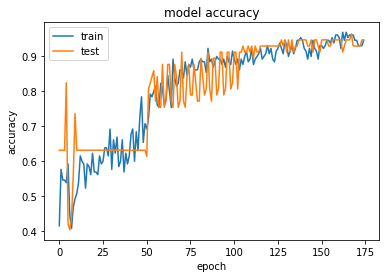
\includegraphics[width=0.5\textwidth]{images/chapter5/batch_256_175_epoch.png}
    \caption{Rendimiento del modelo en acierto usando una gpu TeslaK80 y una configuración de entrenamiento de 175 epoch y un tamaño batch de 256.}
    \label{fig:Resultados de la precisión de entrenamiento con un batch-size de 256 y 175 epochs}
\end{figure}

\begin{figure}
    \centering
    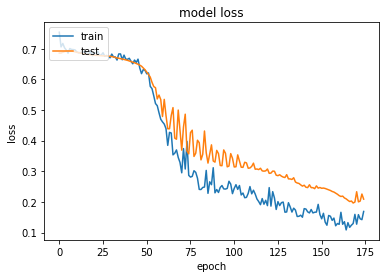
\includegraphics[width=0.5\textwidth]{images/chapter5/batch_256_175_epoch_loss.png}
    \caption{Rendimiento del modelo en pérdida al entrenar con una TeslaK80 y una configuración de entrenamiento de 175 epoch y un tamaño batch de 256.}
    \label{fig:Resultados de loss en el entrenamiento con un batch-size de 256 y 175 epochs}
\end{figure}

\begin{figure}
    \centering
    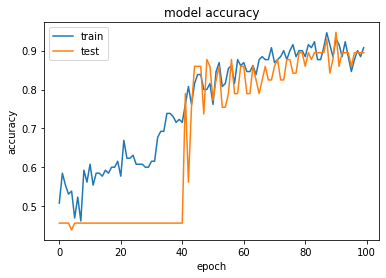
\includegraphics[width=0.5\textwidth]{images/chapter5/batch_256_100_epoch.png}
    \caption{Rendimiento del modelo en acierto usando una gpu TeslaK80 y una configuración de entrenamiento de 100 epoch y un tamaño batch de 256.}
    \label{fig:Resultados de la precisión de entrenamiento con un batch-size de 256 y 100 epochs}
\end{figure}

\begin{figure}
    \centering
    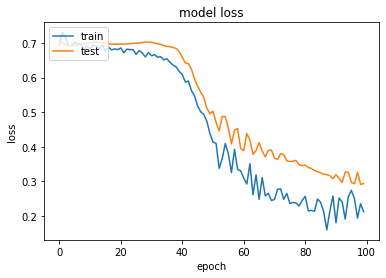
\includegraphics[width=0.5\textwidth]{images/chapter5/batch_256_100_epoch_loss.png}
    \caption{Rendimiento del modelo en pérdida al entrenar con una TeslaK80 y una configuración de entrenamiento de 100 epoch y un tamaño batch de 256.}
    \label{fig:Resultados de loss en el entrenamiento con un batch-size de 256 y 100 epochs}
\end{figure}

\begin{figure}
    \centering
    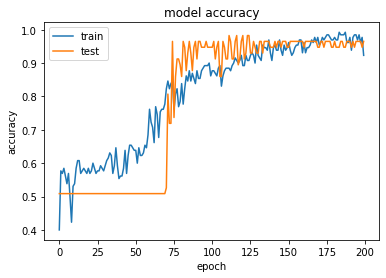
\includegraphics[width=0.5\textwidth]{images/chapter5/batch_256_200_epoch.png}
    \caption{Rendimiento del modelo en acierto usando una gpu TeslaK80 y una configuración de entrenamiento de 200 epoch y un tamaño batch de 256.}
    \label{fig:Resultados de la precisión de entrenamiento con un batch-size de 256 y 200 epochs}
\end{figure}

\begin{figure}
    \centering
    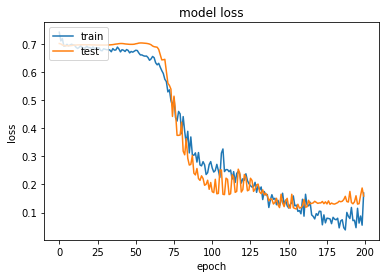
\includegraphics[width=0.5\textwidth]{images/chapter5/batch_256_200_epoch_loss.png}
    \caption{Rendimiento del modelo en pérdida al entrenar con una TeslaK80 y una configuración de entrenamiento de 200 epoch y un tamaño batch de 256.}
    \label{fig:Resultados de loss en el entrenamiento con un batch-size de 256 y 200 epochs}
\end{figure}


\section{Rendimiento en fase de inferencias}\label{sec:ren-dimiento-en-fase-de-inferencias}
En cuanto a los tiempos de inferencia, la diferencia es notable entre OpenVINO y Tensorflow.
Los resultados se presentan haciendo uso de una muestra de 16.000 ejecuciones de inferencia en el entorno de producción de la aplicación, tanto para los entornos con Openvino, como para Tensorflow.
La unidad de cálculo principal es el procesador, siendo su modelo un Intel Xeon (Cascada Lake) con una frecuencia de 2.8 GHz de base y un turbo hasta 3.4 GHz.
Se han probado distintas configuraciones de este procesador, tanto en su versión de 2 núcleos físicos, 4 virtuales como en la de 4 núcleos físicos, 8 virtuales.
La memoria ram utilizada varía de 4 GB en su primera versión junto con el procesador de 2 núcleos físicos a 8 GB en la versión de 4 núcleos físicos.
En la figura~\ref{fig:Comparativa de tiempo de inferencia con OpenVINO y Tensorflow} se puede observar como la media de inferencia a lo largo de las 16.000 muestras tomadas
es de 200ms para Tensorflow y 4ms para OpenVINO lo que supone una velocidad de inferencia 50 veces superior de OpenVINO frente a Tensorflow.
También podemos visualizar en la imagen ~\ref{fig:Comparativa de tiempo de inferencia con OpenVINO y Tensorflow con distinto hardware} que el tiempo total de inferencia,
que incluye la latencia del servidor web, los pipelines de procesamiento del entorno y la propia inferencia es inferior al segundo en ambos casos,
pero muy inferior en OpenVINO debido a la rapidez de su red de inferencia y a la simplicidad con la que se implementa, ya que, al contrario que Tensorflow esta no necesita ningún otro tipo de servicio adicional más
que la API de alto rendimiento que funciona como una librería almacenada de manera local en el sistema operativo.
Las distintas configuraciones hardware también revelan que el consumo de memoria del sistema de inferencia de tensorflow afecta al rendimiento de la aplicación, mejorando mucho su rendimiento con un hardware más potente.
OpenVINO por el contrario mantiene resultados similares con un hardware de bajo coste.
Tensorflow mejora en 5 veces la velocidad de inferencia pasando de un procesador de 2 núcleos y 4 GB de ram a uno de 4 núcleos y 8 GB de ram teniendo un tiempo de 360ms con el primero y 66 con el segundo, lo que denota que el consumo
de su servicio de inferencia requiere de un hardware más caro.
Del mismo modo mejora 8 veces su tiempo de inferencia total con la mejora del hardware pasando de 800ms a 97ms.
\begin{figure}
    \centering
    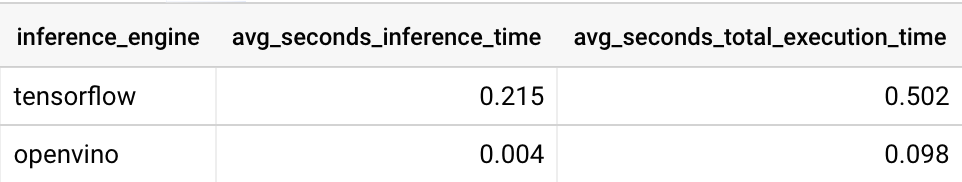
\includegraphics[width=0.8\textwidth]{images/chapter5/time_inference_engine.png}
    \caption{Comparativa de tiempos de inferencia con OpenVINO y Tensorflow}
    \label{fig:Comparativa de tiempo de inferencia con OpenVINO y Tensorflow}
\end{figure}

\begin{figure}
    \centering
    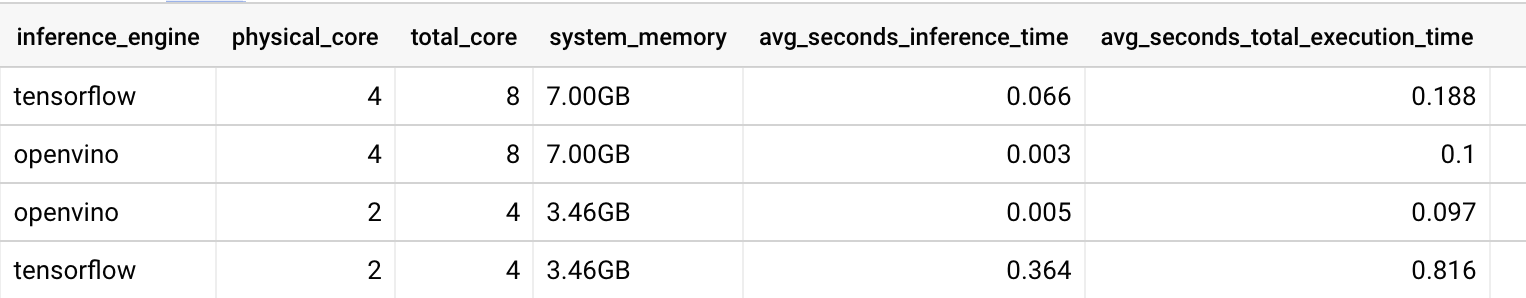
\includegraphics[width=0.8\textwidth]{images/chapter5/time_inference_system_engine.png}
    \caption{Comparativa de tiempos de inferencia con OpenVINO y Tensorflow con distinto hardware}
    \label{fig:Comparativa de tiempo de inferencia con OpenVINO y Tensorflow con distinto hardware}
\end{figure}

La puesta a prueba de los distintos servidores web se ha llevado a cabo mediante la configuracion de estos para trabajar de manera concurrente usando todos los núcleos del
procesador, de modo que la capacidad de procesamiento de peticiones sea la máxima posible.
En la figura~\ref{fig:Comparativa de tiempo de inferencia con OpenVINO y Tensorflow con distinto framework web} podemos contemplar que OpenVINO se mantiene estable con ambos framework, con un ligero aumento de la latencia haciendo uso de fastapi.
Tensorflow se comporta mucho mejor con flask, mejorando en 4 veces su tiempo de inferencia en la red, pasando de 348ms con fastapi a 83ms con flask y 3.7 veces en el tiempo total de ejecución teniendo un rendimiento de 700ms con fastapi a 200ms con flask.
Flask es un servidor web con los mínimos componentes para funcionar, pero configurado de la manera correcta puede ser el framework perfecto para realizar una tarea específica, en este caso
la complejidad del servicio de Tensorflow convive mejor con un framework web sin demasiados componentes adicionales.
Es cierto que los componentes que proporciona fastapi como un sistema de logging detallado de las ejecuciones y algunas características adicionales
para el desarrollador pueden causar cierto aumento de la latencia en los tiempos, pero cuando la fiabilidad es uno de los requisitos y objetivos principales estas mejoras
pueden valer la pena a la hora de escalar nuestra aplicación.
En general, fastapi requiere de un hardware más potente para sacar su máximo rendimiento, mientras que con una framework minimalista como flask podemos optar por reducir costes en hardware sin penalizar demasiado
el rendimiento.
En la figura~\ref{fig:Comparativa de tiempo de inferencia con OpenVINO y Tensorflow con distinto hardware y servidor web} podemos ver el rendimiento según hardware, servidor web y sistema de inferencia utilizado.

\begin{figure}
    \centering
    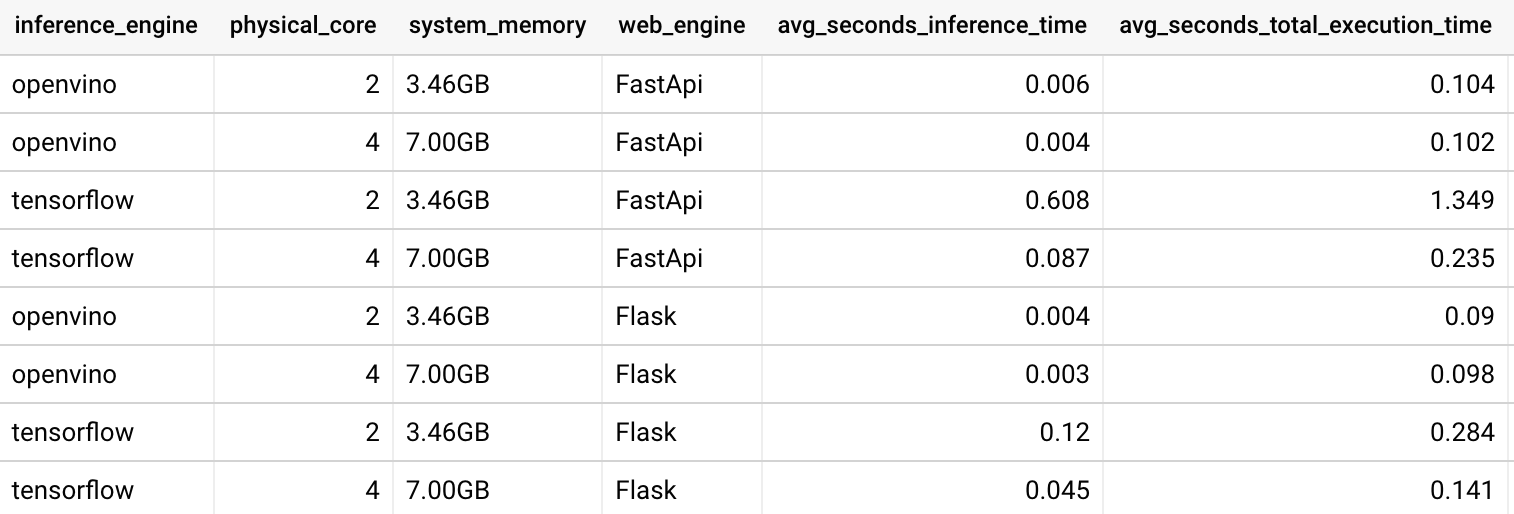
\includegraphics[width=0.8\textwidth]{images/chapter5/time_general.png}
    \caption{Comparativa de tiempos de inferencia con OpenVINO y Tensorflow con distinto hardware y servidor web}
    \label{fig:Comparativa de tiempo de inferencia con OpenVINO y Tensorflow con distinto hardware y servidor web}
\end{figure}



\begin{figure}
    \centering
    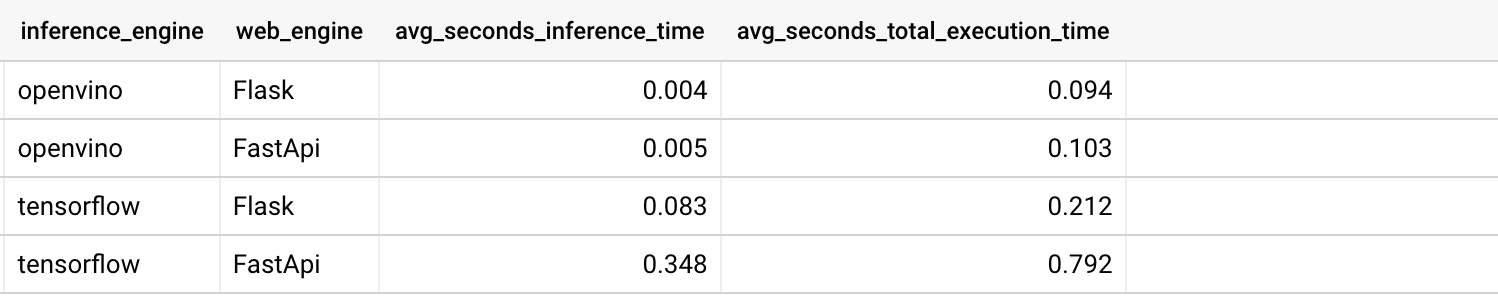
\includegraphics[width=0.8\textwidth]{images/chapter5/time_inference_web.png}
    \caption{Comparativa de tiempos de inferencia con OpenVINO y Tensorflow con distinto framework web}
    \label{fig:Comparativa de tiempo de inferencia con OpenVINO y Tensorflow con distinto framework web}
\end{figure}

El número total de aciertos de clasificación en ambas redes asciende a 1566 registros de un total de 16000, teniendo así un porcentaje de acierto general
del 97 por ciento.Con un recuento de 108 fallos en la red tensorflow y 226 en openvino.
Todos los resultados y registros se encuentran en el repositorio oficial del trabajo en Github\footnote{https://github.com/A-Ortiz-L/multispectral-imaging-cnn-final-degree-work/tree/master/result/snapshot}


\section{Costes del proyecto}\label{sec:costes-del-proyecto}
A continuación se presentan los costes del proyecto de toda la plataforma de producción.
Estos costes han sido recogidos haciendo uso de la calculadora de precios de google\footnote{https://cloud.google.com/products/calculator?hl=es}

\begin{itemize}
    \item Máquina virtual 4 vCPUs, 3,6 GB 6.80 dólares por un uso de 24 horas, que fue el tiempo utilizado para realizar pruebas de concepto y cargas en este trabajo.
    \item Máquina virtual 4 vCPUs, 3,6 GB 3.40 dólares por un uso de 24 dólares, que fue el tiempo real consumido para este servicio.
    \item BigQuery, con un coste de 0 dólares para un almacenamiento de 1 GB de tablas en la base de datos, 1GB de procesamiento en tiempo real y 1GB de trabajos SQL al realizar los análisis de resultados.
    \item Pub/Sub con un coste total de 0 dólares, ya que su uso entraba dentro del rango gratuito del servicio.
    \item Cloud Functions, con un coste total de 0 dólares, haciendo uso de la modalidad gratuita, que permite hasta 2 millones de llamadas al mes.
\end{itemize}

